\documentclass[a4paper, 12pt]{article}
% math symbols
\usepackage{amssymb}
\usepackage{amsmath}
\usepackage{mathrsfs}
\usepackage{physsummer}


\usepackage{enumitem}
\usepackage[margin = 2cm]{geometry}

\tolerance = 1000
\emergencystretch = 0.74cm



\pagestyle{empty}
\parindent = 0mm

\renewcommand{\libproblempath}{../../../materials/problems_db}

\begin{document}

\setphysstyle{ГЦФО 9}{Серия Ш-05}{18.10.2017}
\setcounter{notask}{13}

\Large


\taskpic{ Точка движется вдоль оси $x$. График зависимости скорости от
  координаты представлен на рисунке~---~он представляет собой дугу
  окружности. Найдите время перемещения от $0$ до $x_0$ и ускорение
  при приближении к точке $x_0$. }
{
  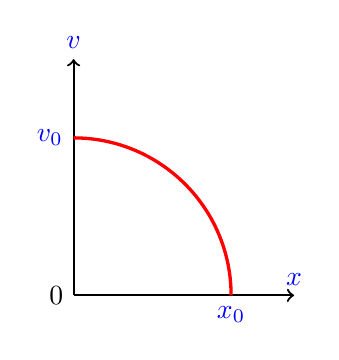
\begin{tikzpicture}
    \draw[thick,->] (0,0) node[left] {0} -- (2.8,0) node[above,blue] {$x$};
    \draw[thick,->] (0,0) -- (0,3) node[above,blue] {$v$};
    \draw[very thick, red] (0,2) node[left,blue] {$v_0$} arc
    (90:0:2cm) node[below,blue] {$x_0$}; 
  \end{tikzpicture}
}
% Зильберман, 1.34


\task{ Диск радиуса $R$ помещён между двумя параллельными
  рейками. Рейки движутся со скоростями $v_1$ и $v_2$. Определить
  угловую скорость вращения диска и скорость его
  центра. Проскальзывание отсутствует. }
% Квант-1972-09, Асламазов, стр. 57

\task{ Маятник Фуко является наглядной иллюстрацией суточного вращения
  Земли. Он представляет собой гладкий тяжёлый шар, подвешенный на
  длинной нерастяжимой нити. Известно, что плоскость его колебаний
  непрерывно поворачивается с некоторой угловой скоростью $\omega$,
  зависящей от широты места установки маятника $\phi$. Связано это с
  тем, что относительно гелиоцентрической системы отсчёта Земля
  вращается вокруг собственной оси с периодом $T$. Найдите угловую
  скорость вращения плоскости колебаний маятника Фуко относительно
  Земли в зависимости от широты.  }
% Паршаков


\end{document}

%%% Local Variables: 
%%% mode: latex
%%% TeX-engine:xetex
%%% TeX-PDF-mode: t
%%% End:
